\documentclass{article}
\usepackage[utf8]{inputenc}
\usepackage{graphicx}

\title{Laporan Tugas Database 2}
\author{Dian Markuci (1184095)}
\date{1 November 2019}

\begin{document}

\maketitle

\section {\textbf Langkah-langkah Membuat Aplikasi di Oracle Express}\\

\item 1. Login 
\begin{center}
    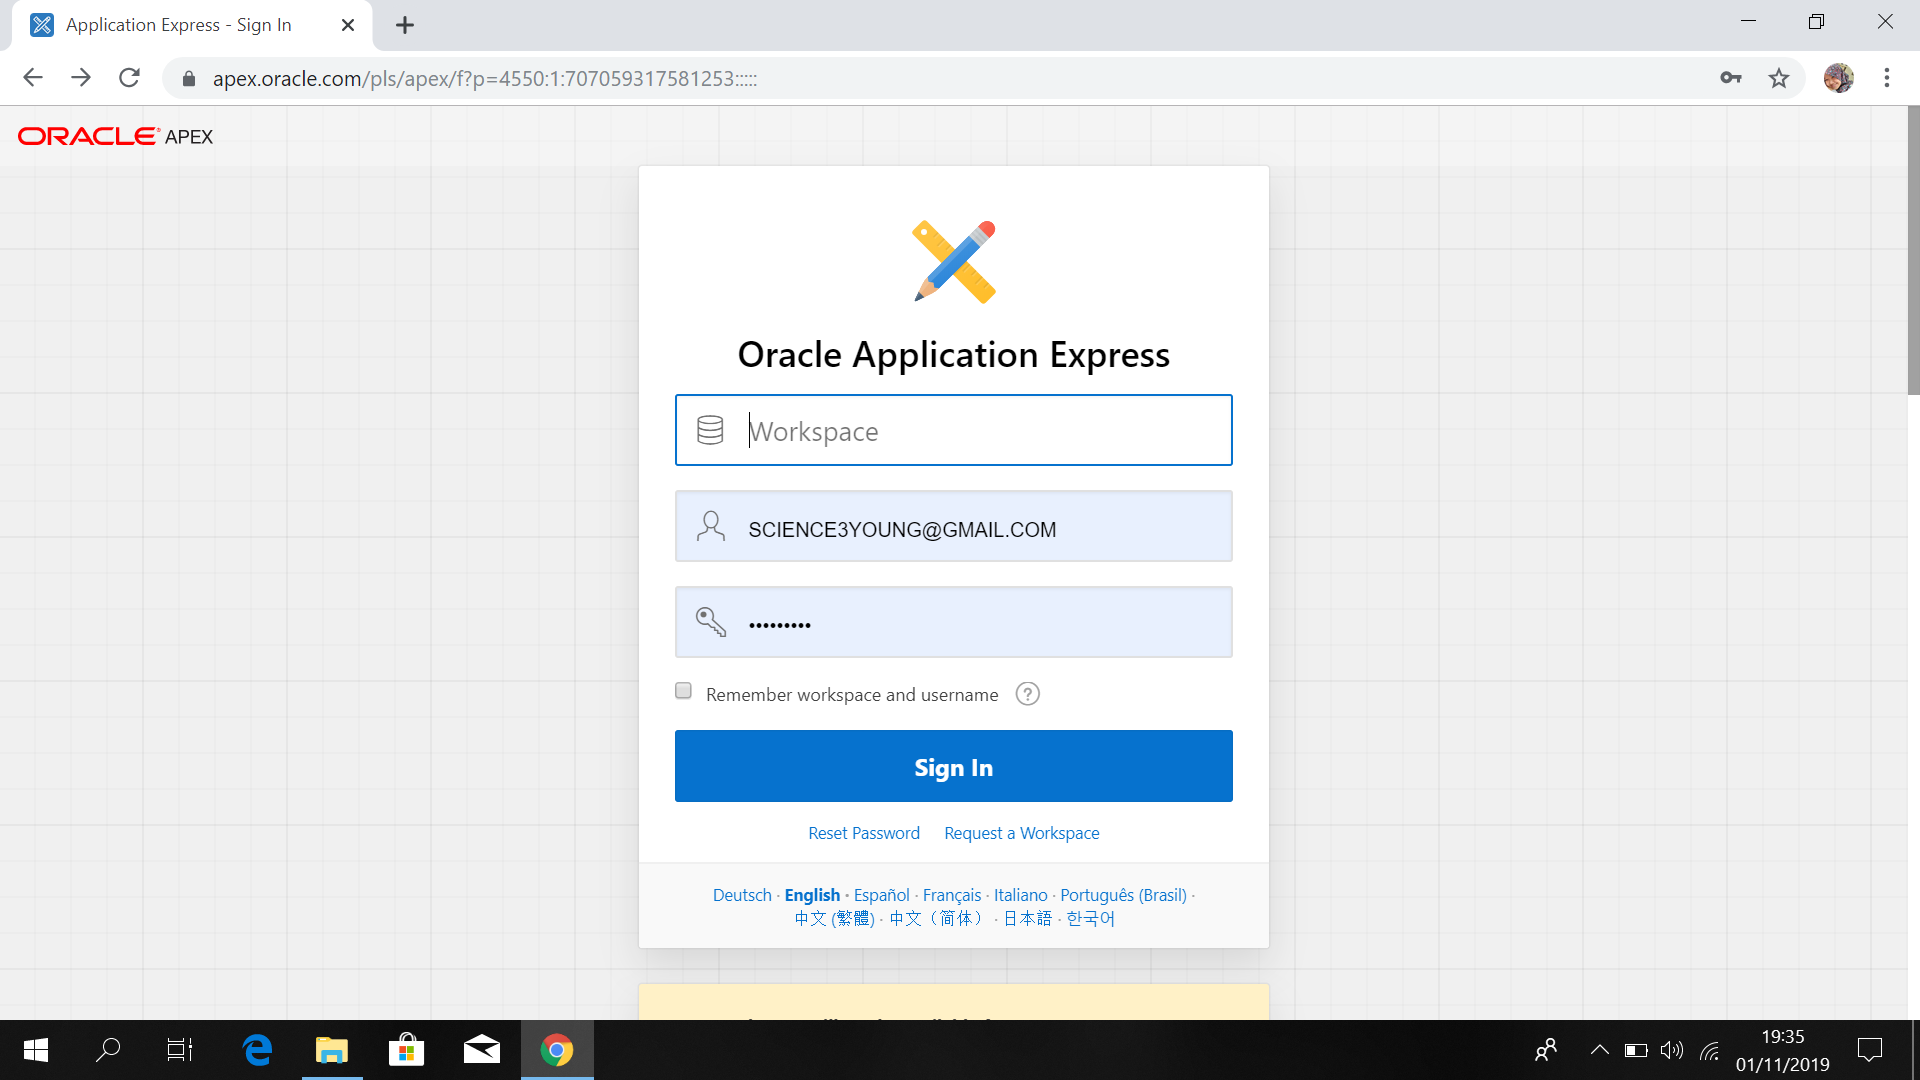
\includegraphics[width=10cm\textwidth]{figure/1login.png}
\end{center}\\

\item 2.Pilih App Builder
\begin{center}
    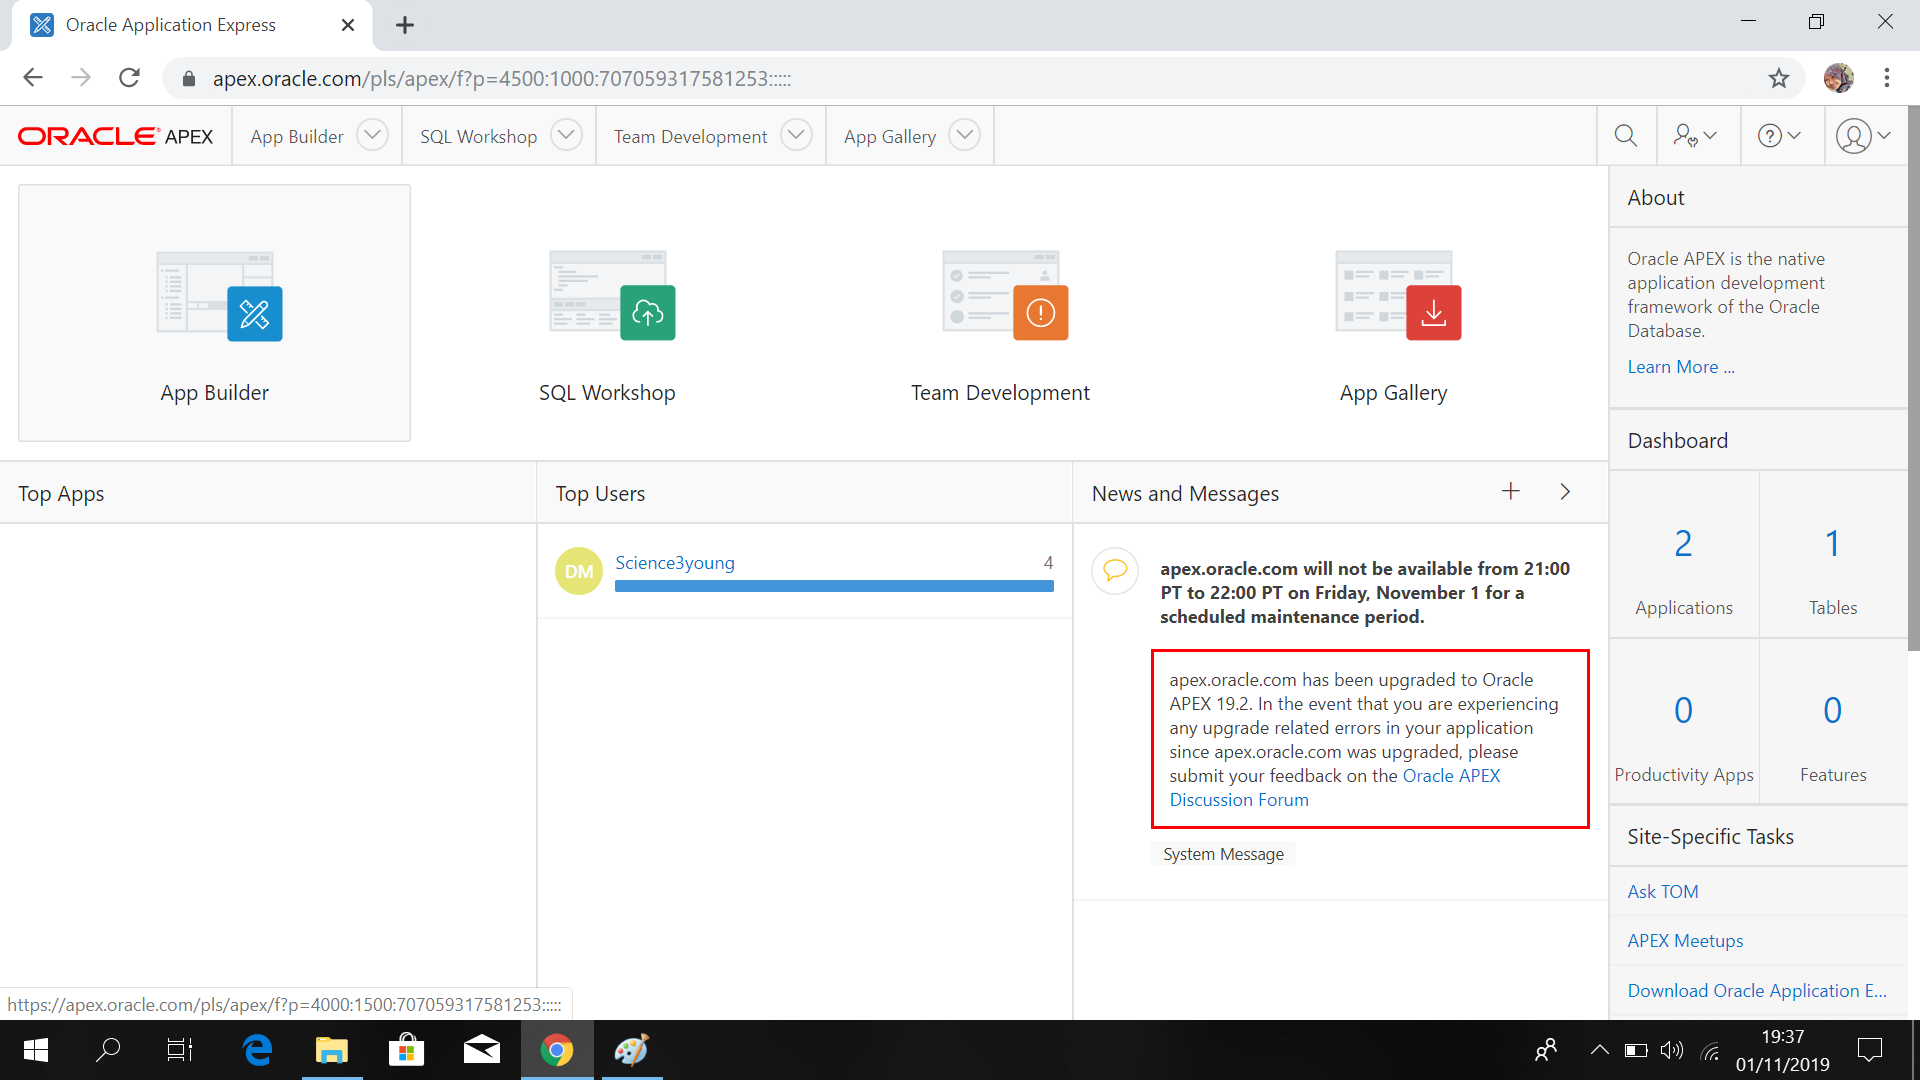
\includegraphics[width=10cm\textwidth]{figure/2Appbuilder.png}\\
\end{center}

\item 3. pilih data dari pc/laptop, lalu pilih create
\begin{center}
    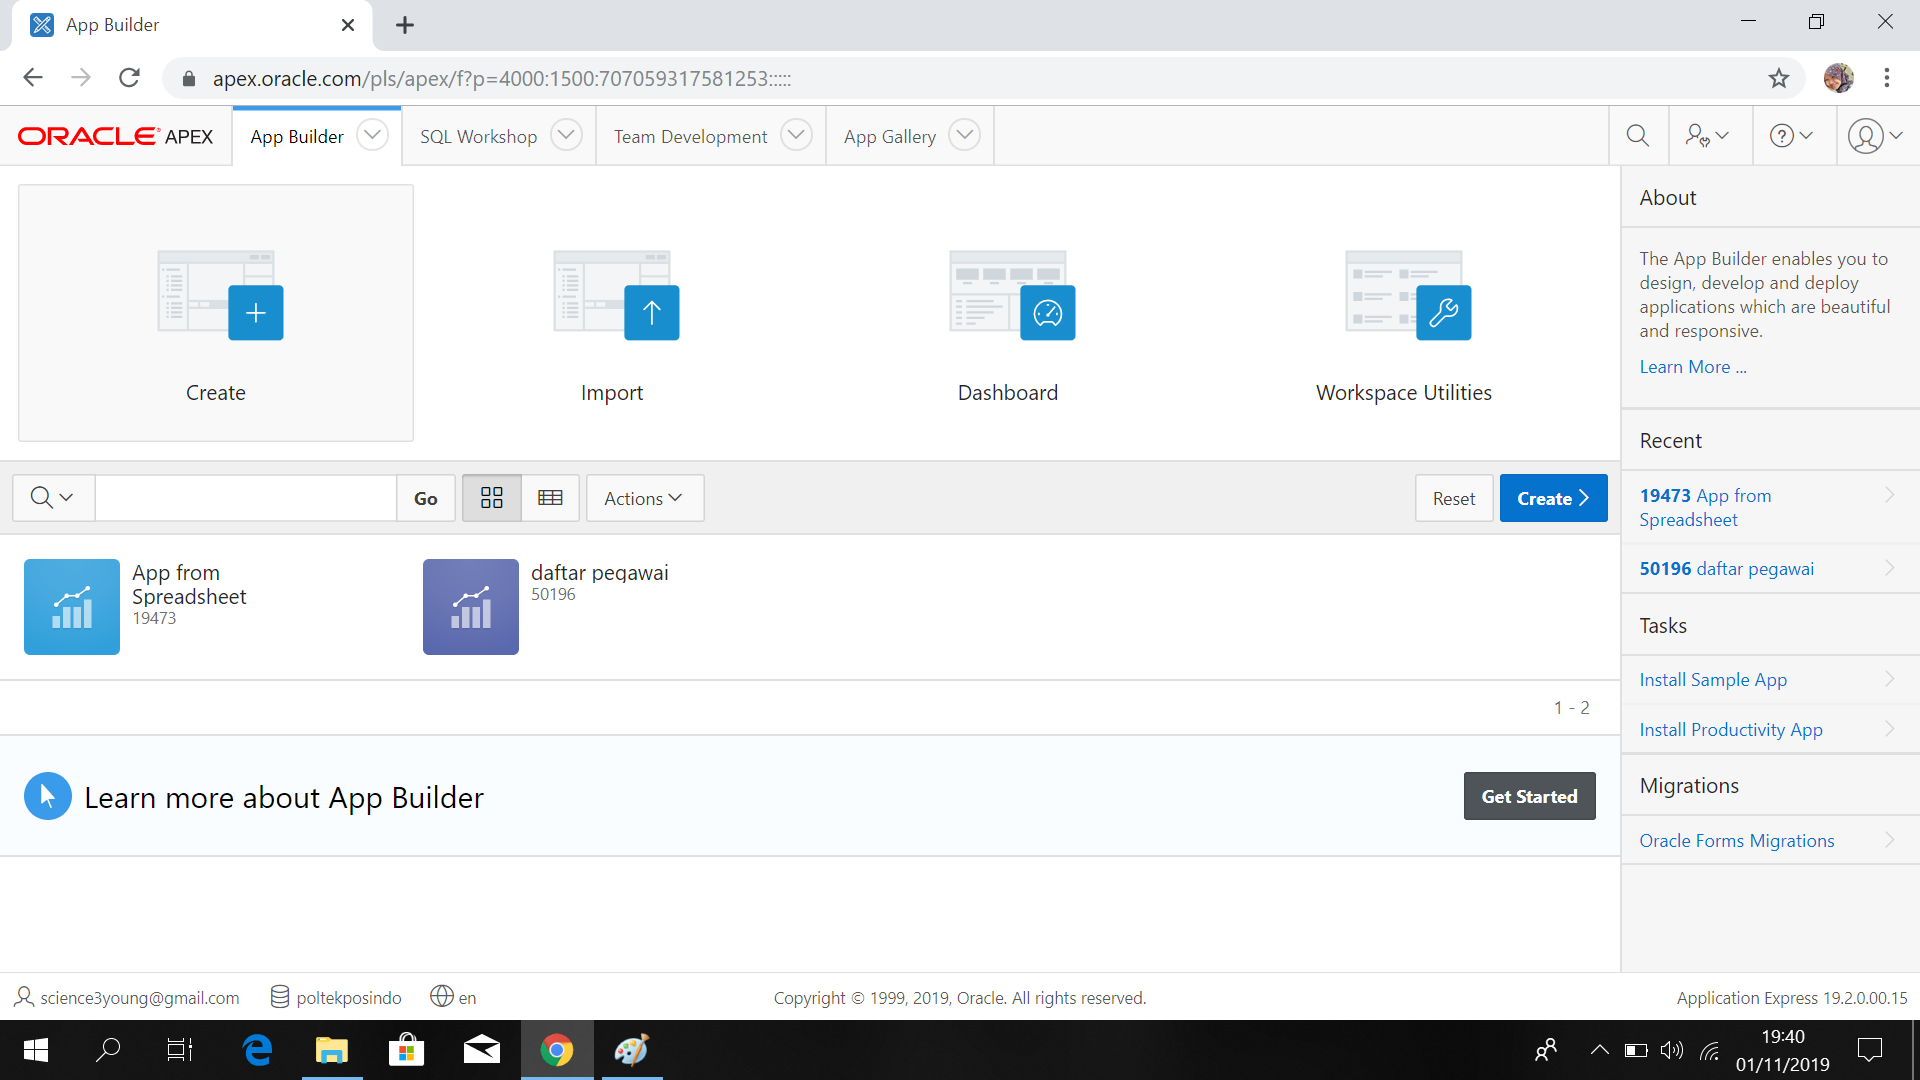
\includegraphics[width=10cm\textwidth]{figure/3Create.png}\\
\end{center}

\item 4. Pilih from a file 
\begin{center}
    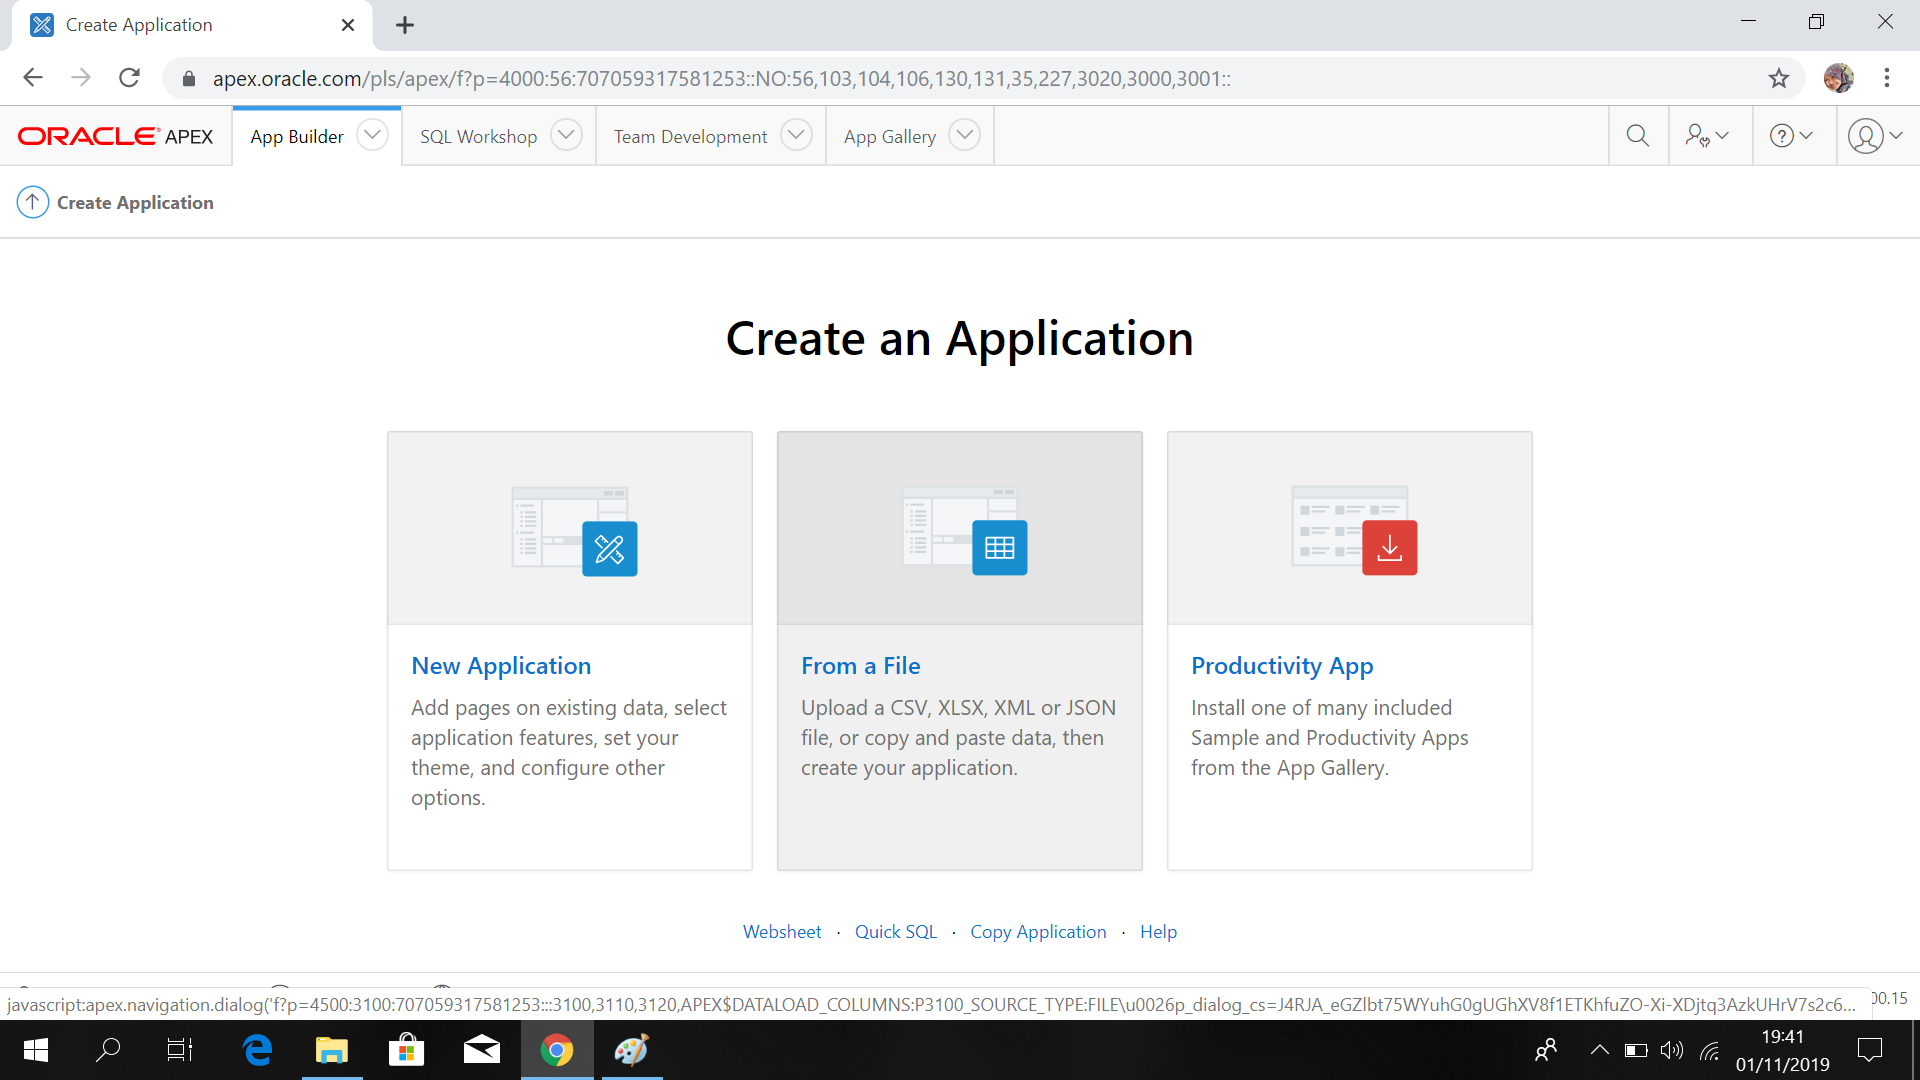
\includegraphics[width=10cm\textwidth]{figure/4from.png}\\
\end{center}

\item 5. klik choose file
\begin{center}
    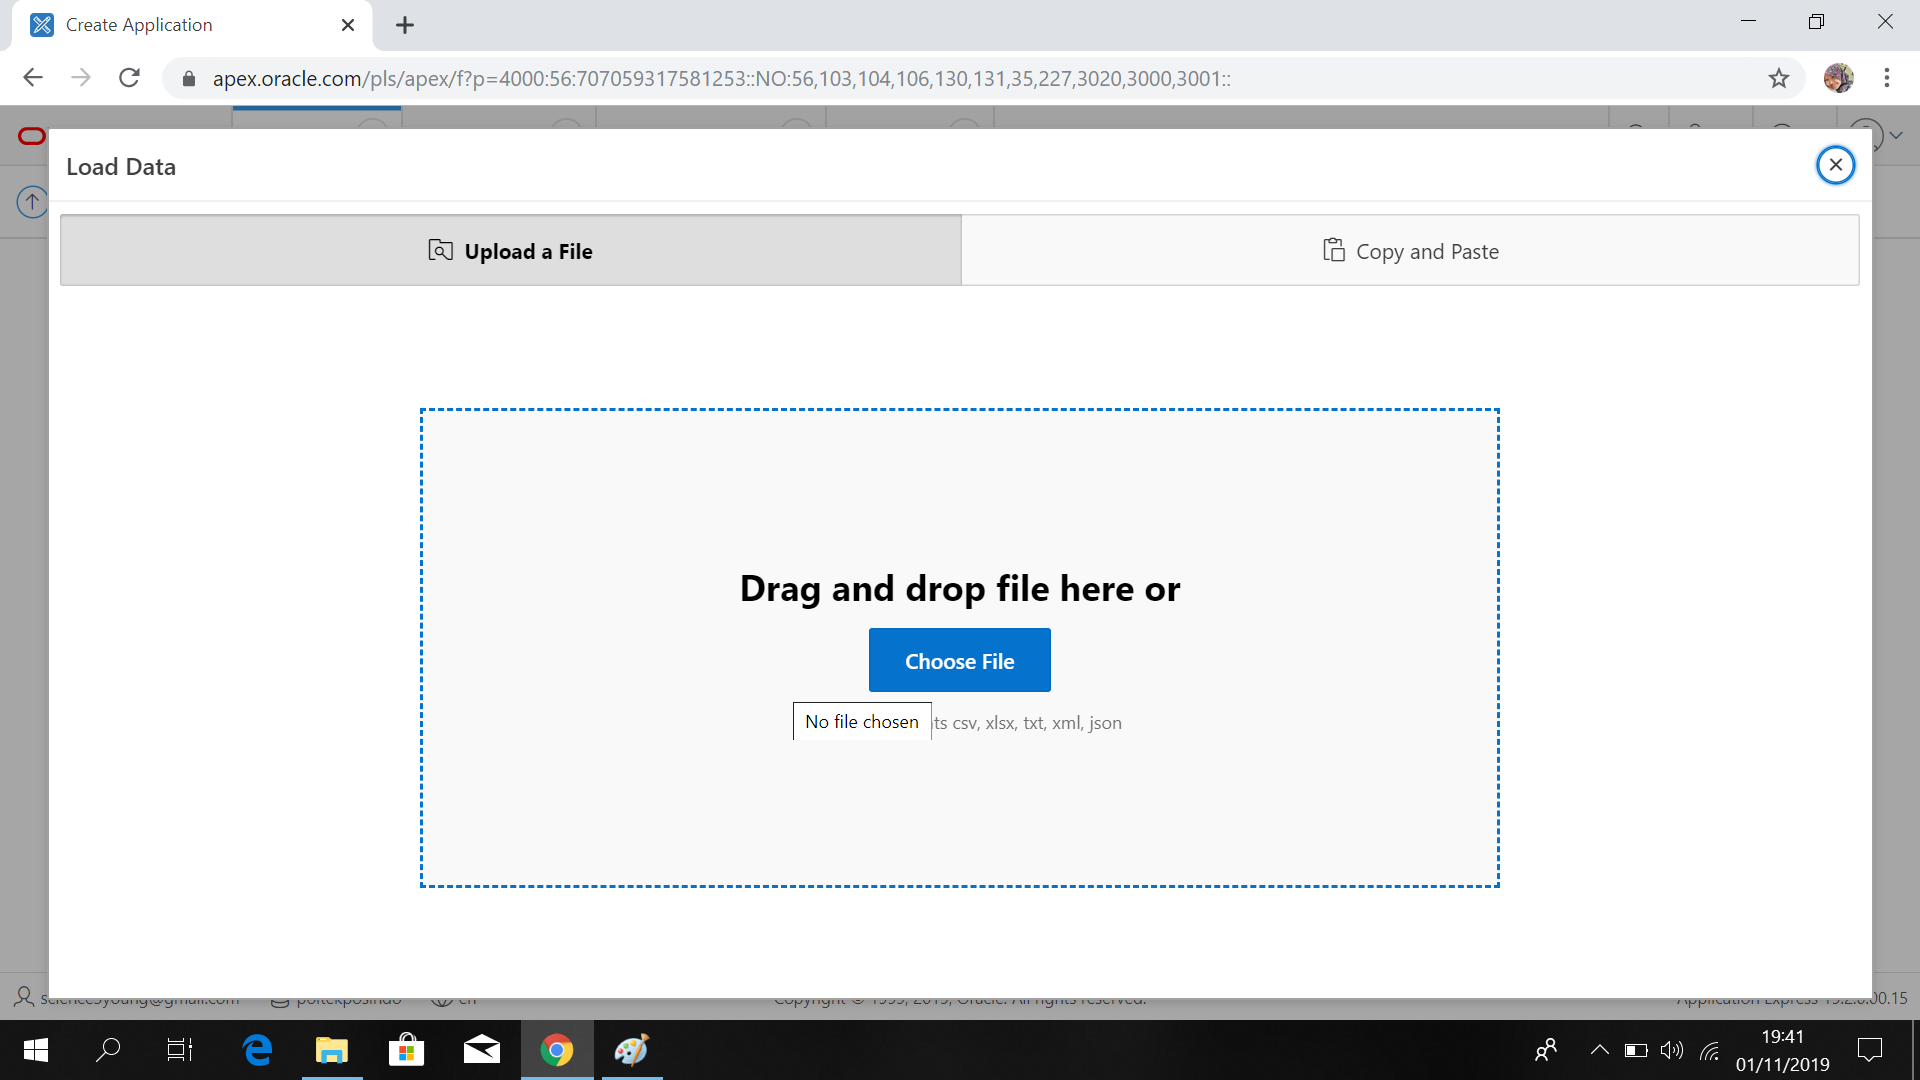
\includegraphics[width=10cm\textwidth]{figure/5choose.png}
    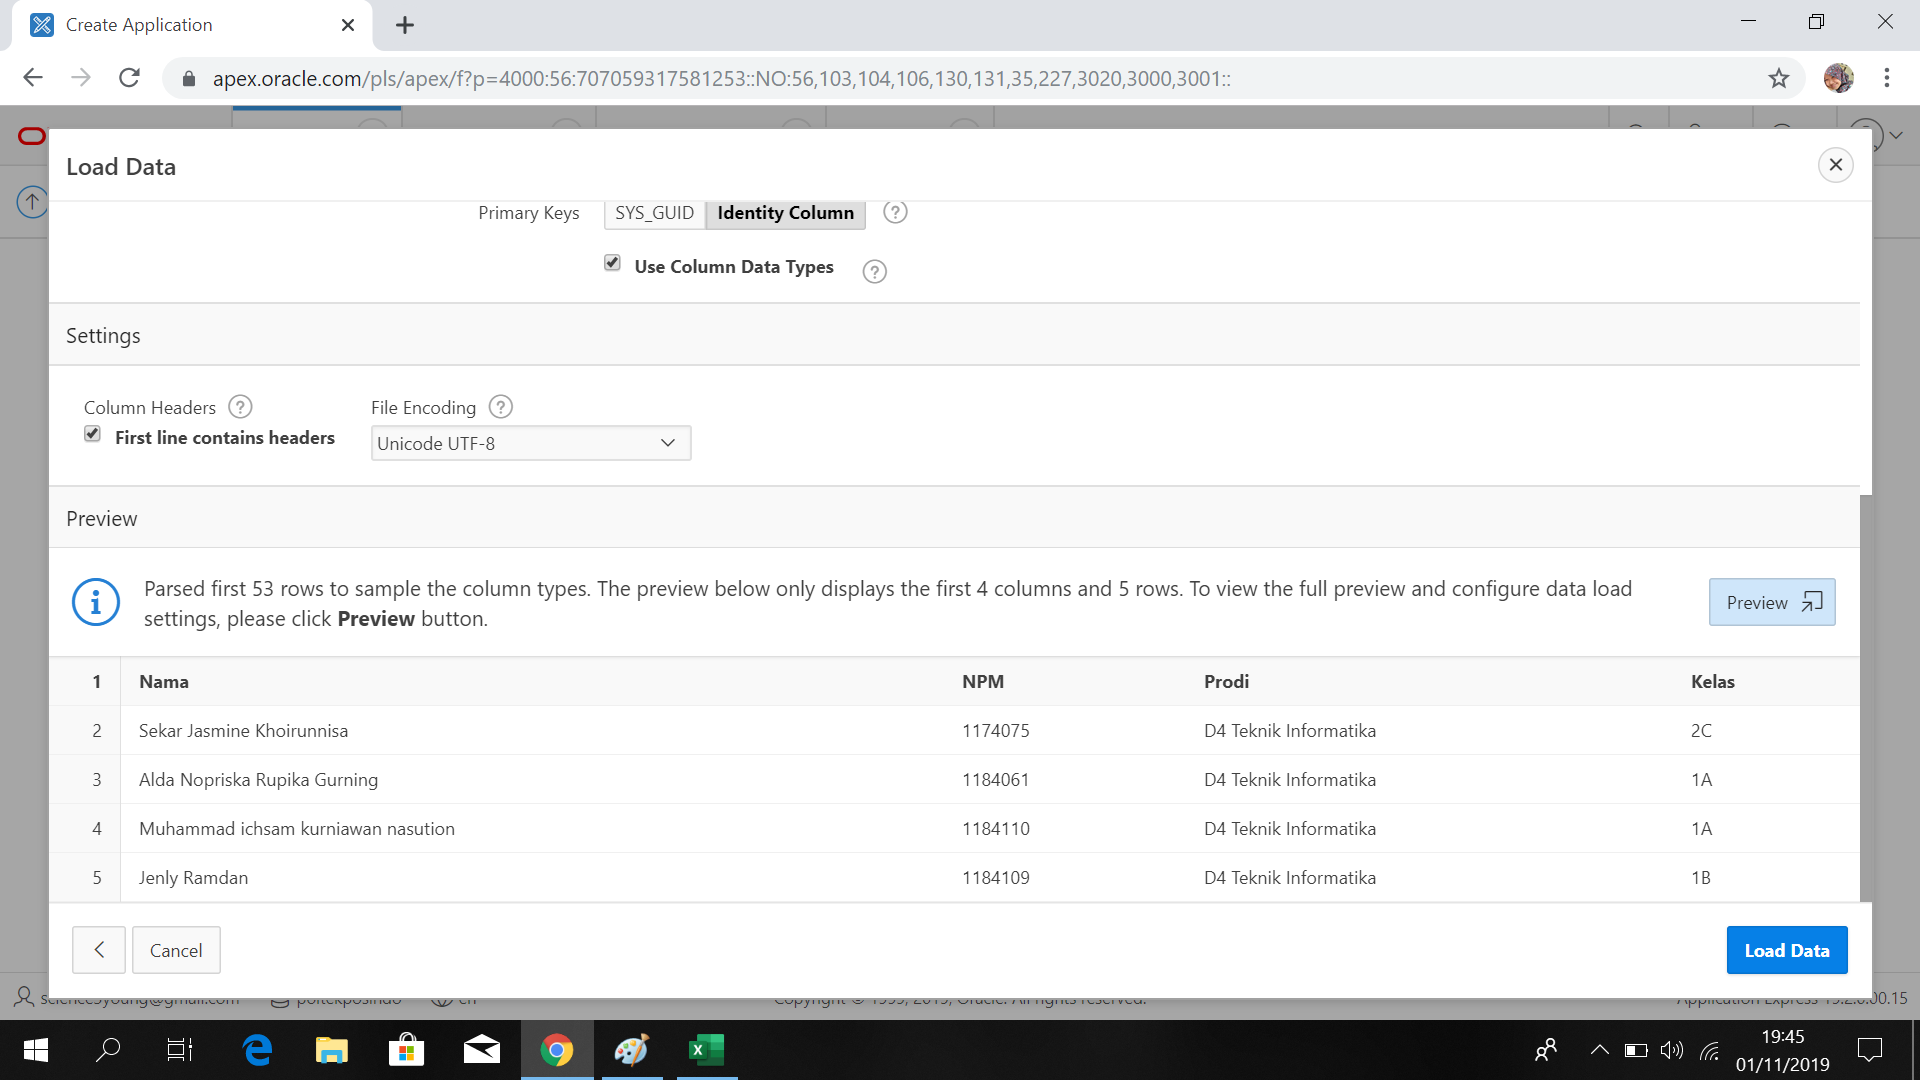
\includegraphics[width=10cm\textwidth]{figure/6load.png}
    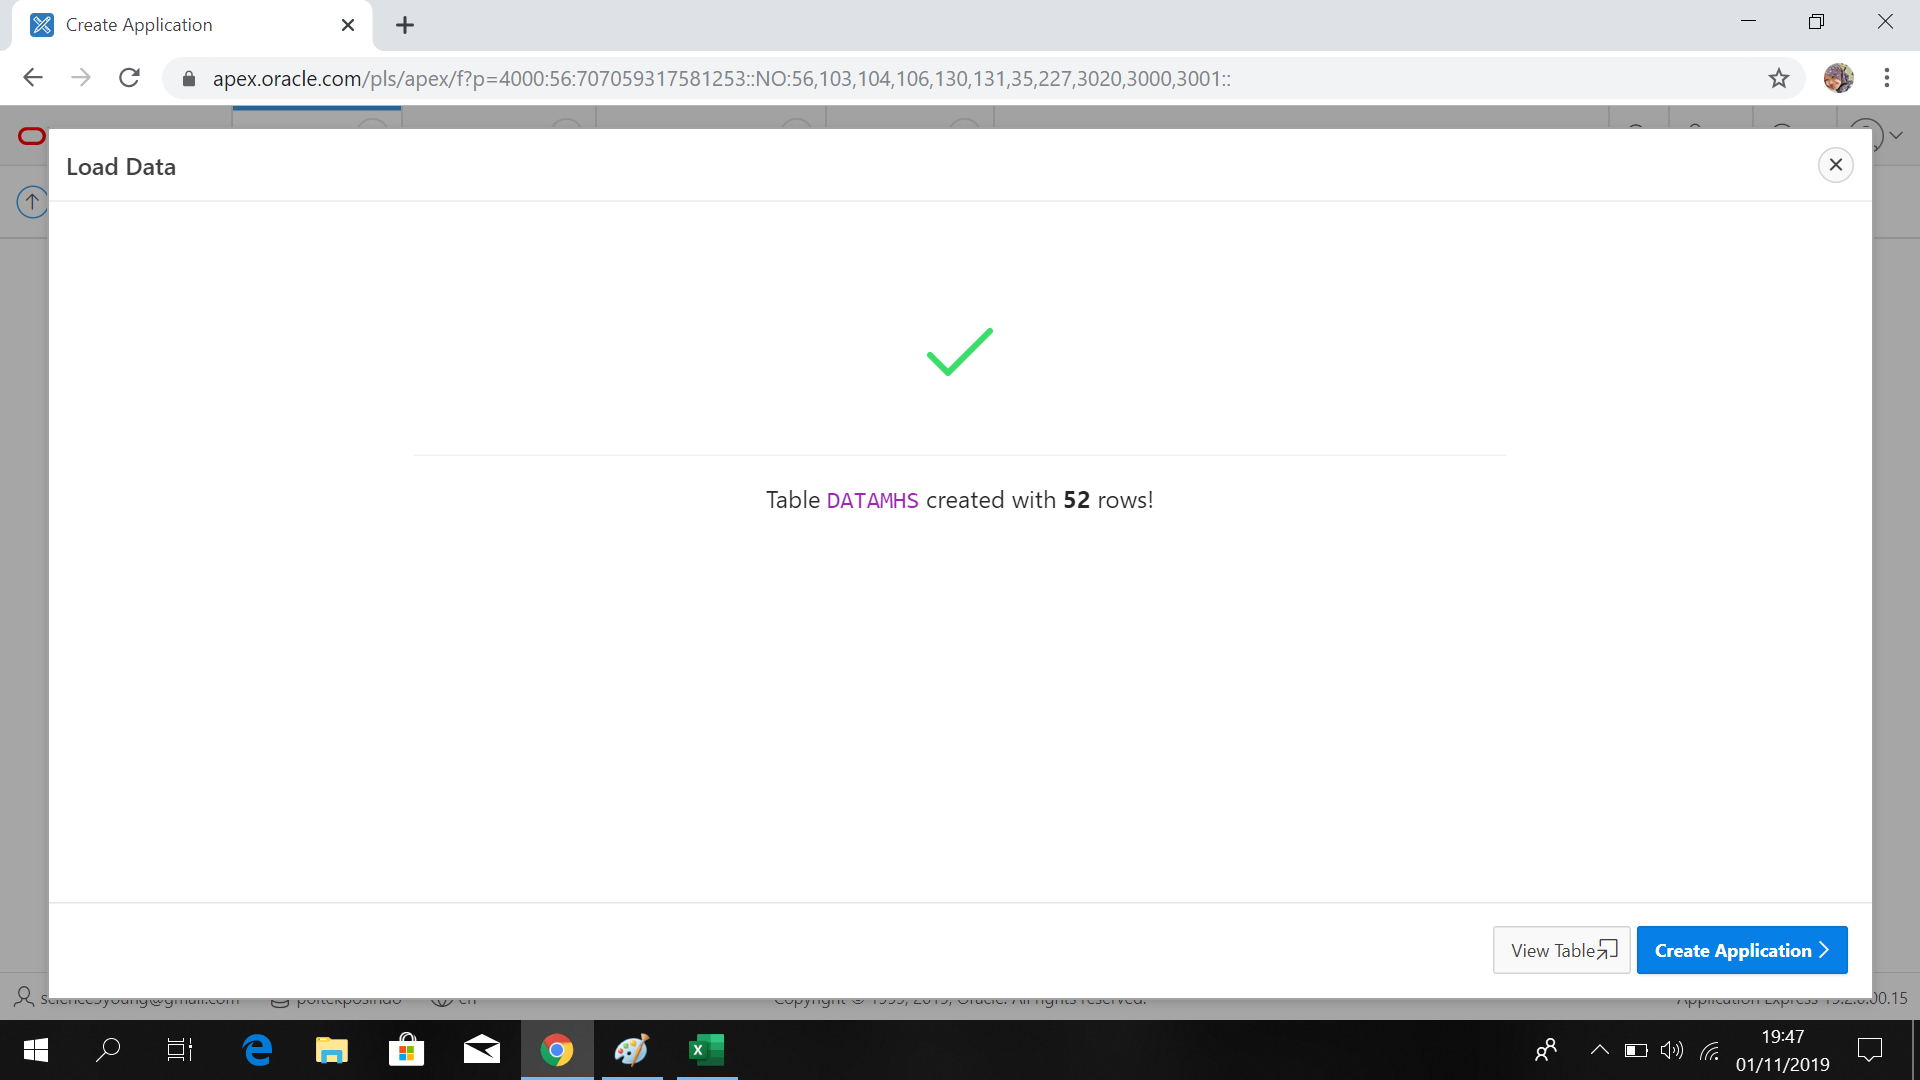
\includegraphics[width=10cm\textwidth]{figure/7create.png}
\end{center}

\item 6. Jangan lupa di cek all
\begin{center}
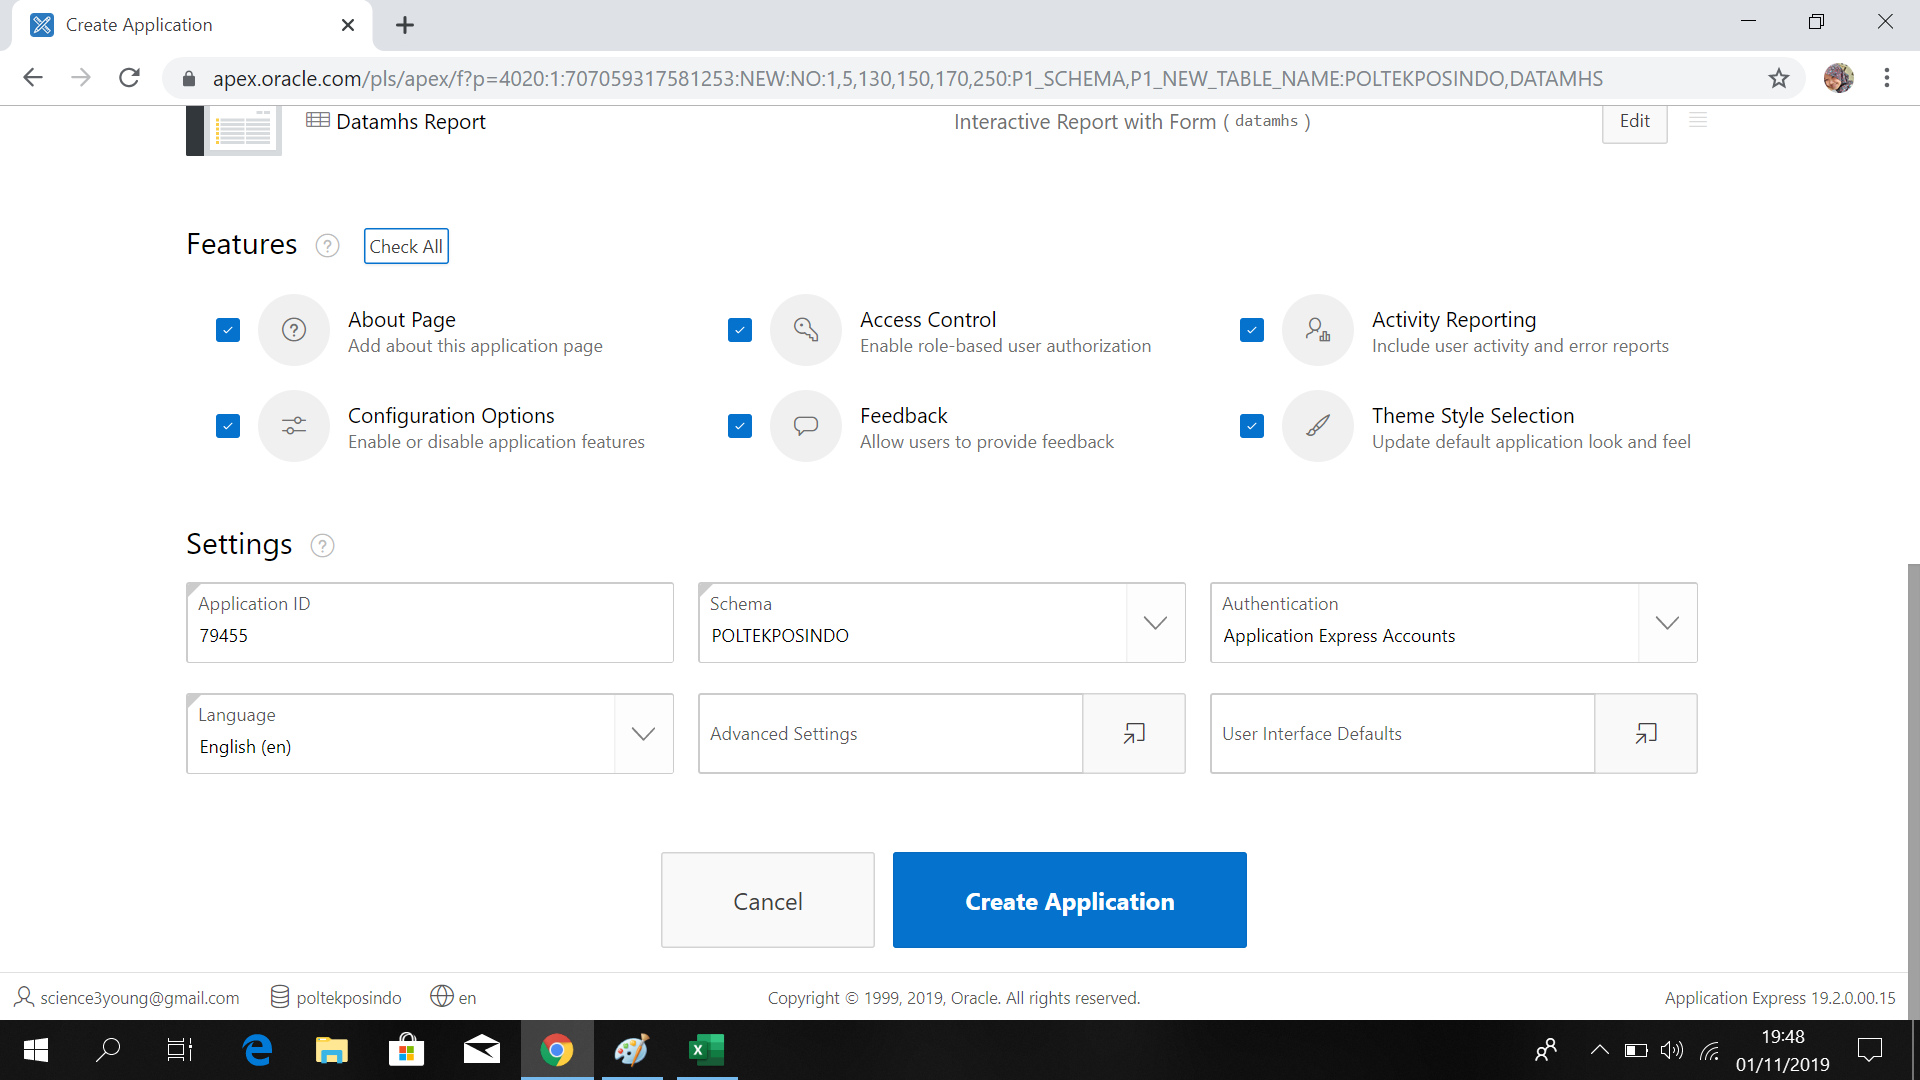
\includegraphics[width=10cm\textwidth]{figure/8chekall.png}
\end{center}

\item 7. run app
\begin{center}
    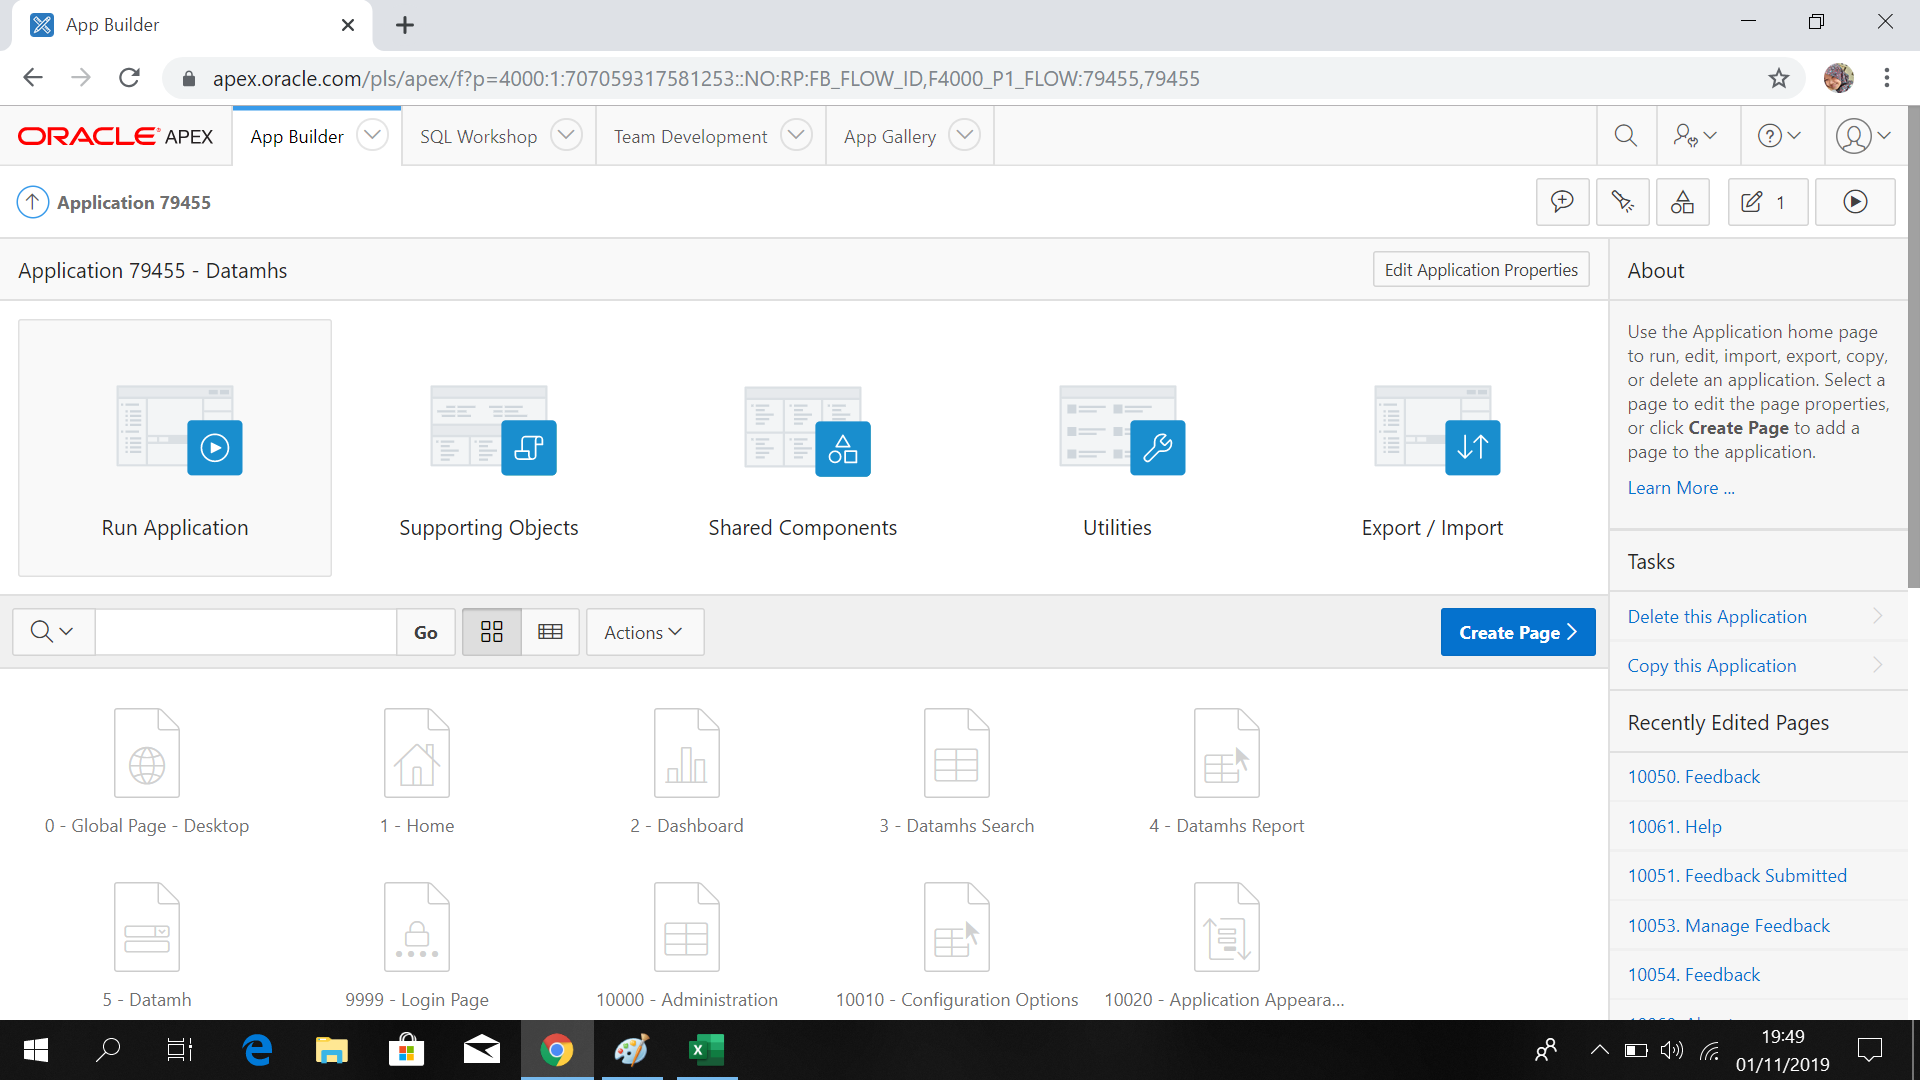
\includegraphics[width=10cm\textwidth]{figure/9run.png}
\end{center}

\item \textbf{SELESAI}

workspace: poltekposindo\\
username : science3young@gmail.com\\
password : dialine31\\
\end{document}


